\subsection{Red Hogareña}

En este experimento, capturamos los paquetes de la LAN hogareña de uno de los miembros de nuestro grupo. La medición fue realizada un día sábado desde las 12 hs hasta las 14 hs. La cantidad de paquetes capturados aproximadamente es de 125000. Sin embargo, sólo 153 de estos corresponden al protocolo ARP.

\begin{figure}[H]
       \centering
       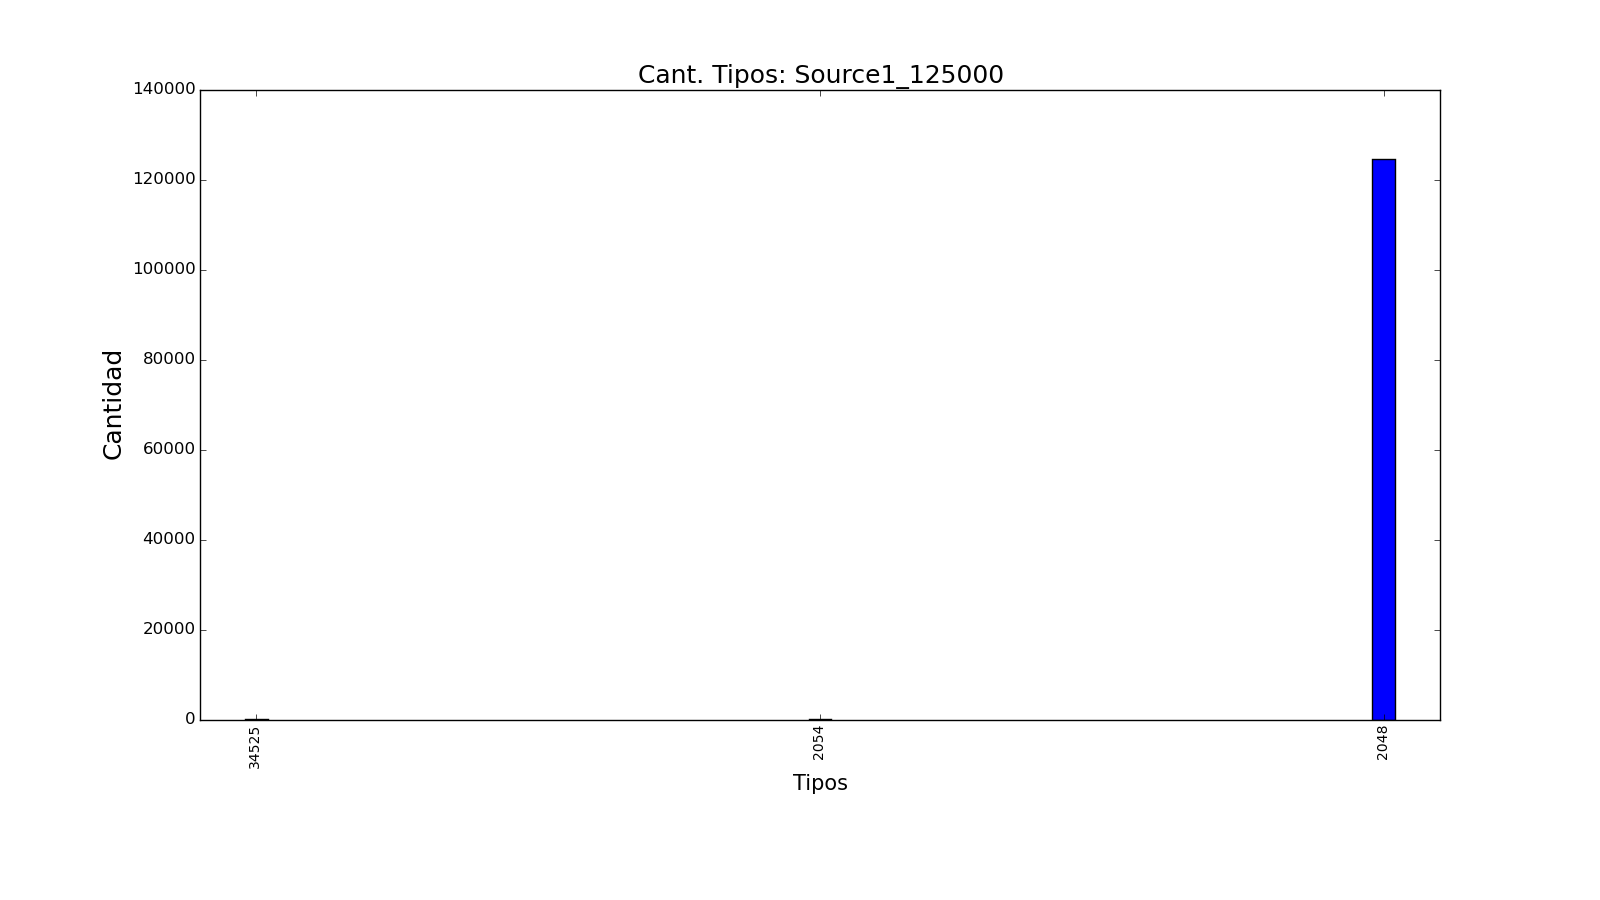
\includegraphics[width=1\textwidth]{../resultados/Casa/histogram_types.png}
       \caption{Protocolos de los paquetes capturados}
       \label{red-hogarena-types}
\end{figure}

\begin{figure}[H]
       \centering
       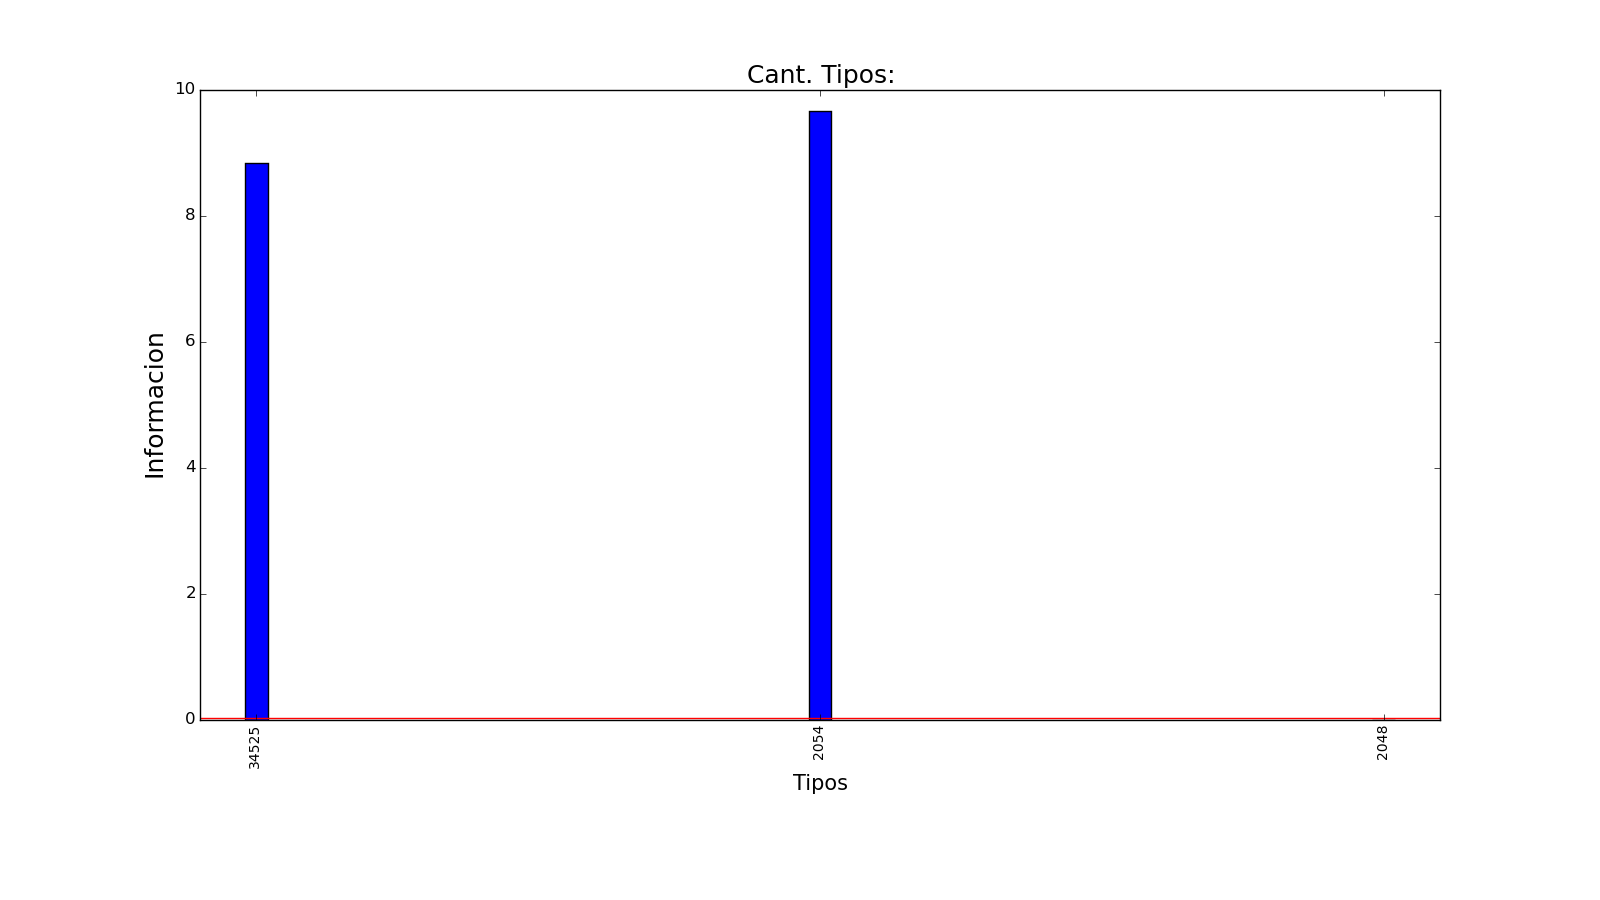
\includegraphics[width=1\textwidth]{../resultados/Casa/histogram_types_information.png}
       \caption{Información de los protocolos de los paquetes capturados}
       \label{red-hogarena-types-info}
\end{figure}

Como podemos observar, de acuerdo a la definición de protocolo distinguido que dimos anteriormente, el protocolo IPv4 sería el único distinguido en esta fuente. Esto resulta razonable, ya que la cantidad de paquetes IPv4 es mucho mayor que la cantidad de paquetes IPv6 y ARP. La información de los paquetes IPv4 es \textbf{0.00491352086592}, mientras que la entropía de la fuente es \textbf{0.0359827861687}. Se observa claramente como la información es menor a la entropía.


\begin{figure}[H]
       \centering
       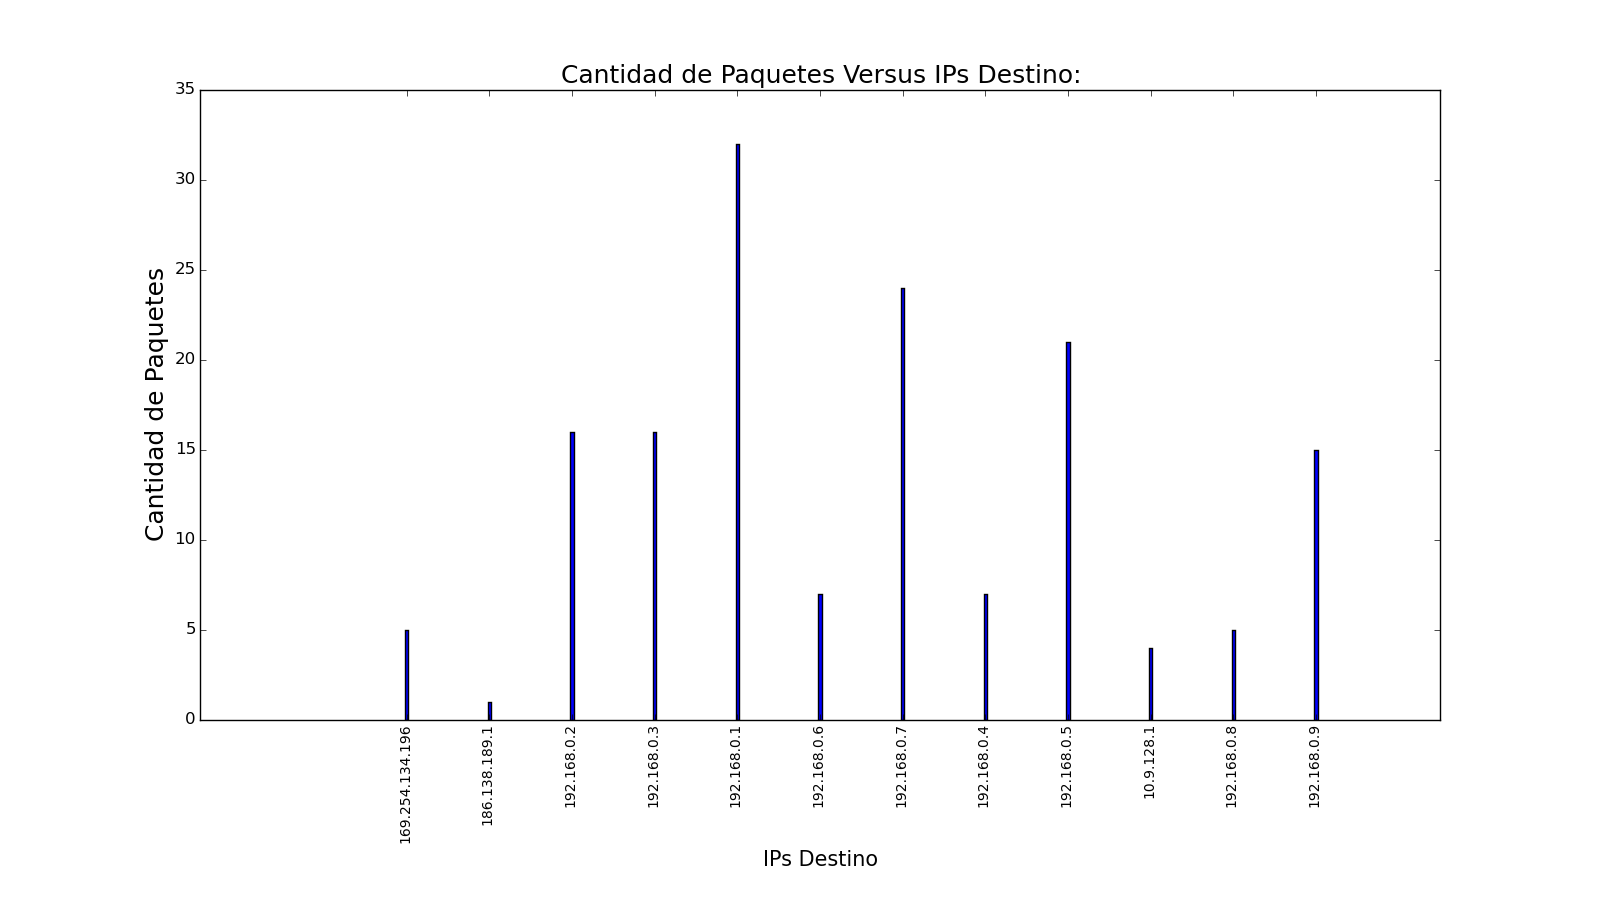
\includegraphics[width=1\textwidth]{../resultados/Casa/histogram_dst.png}
       \caption{IPs destino de los paquetes ARP}
       \label{red-hogarena-arp-destination}
\end{figure}

\begin{figure}[H]
       \centering
       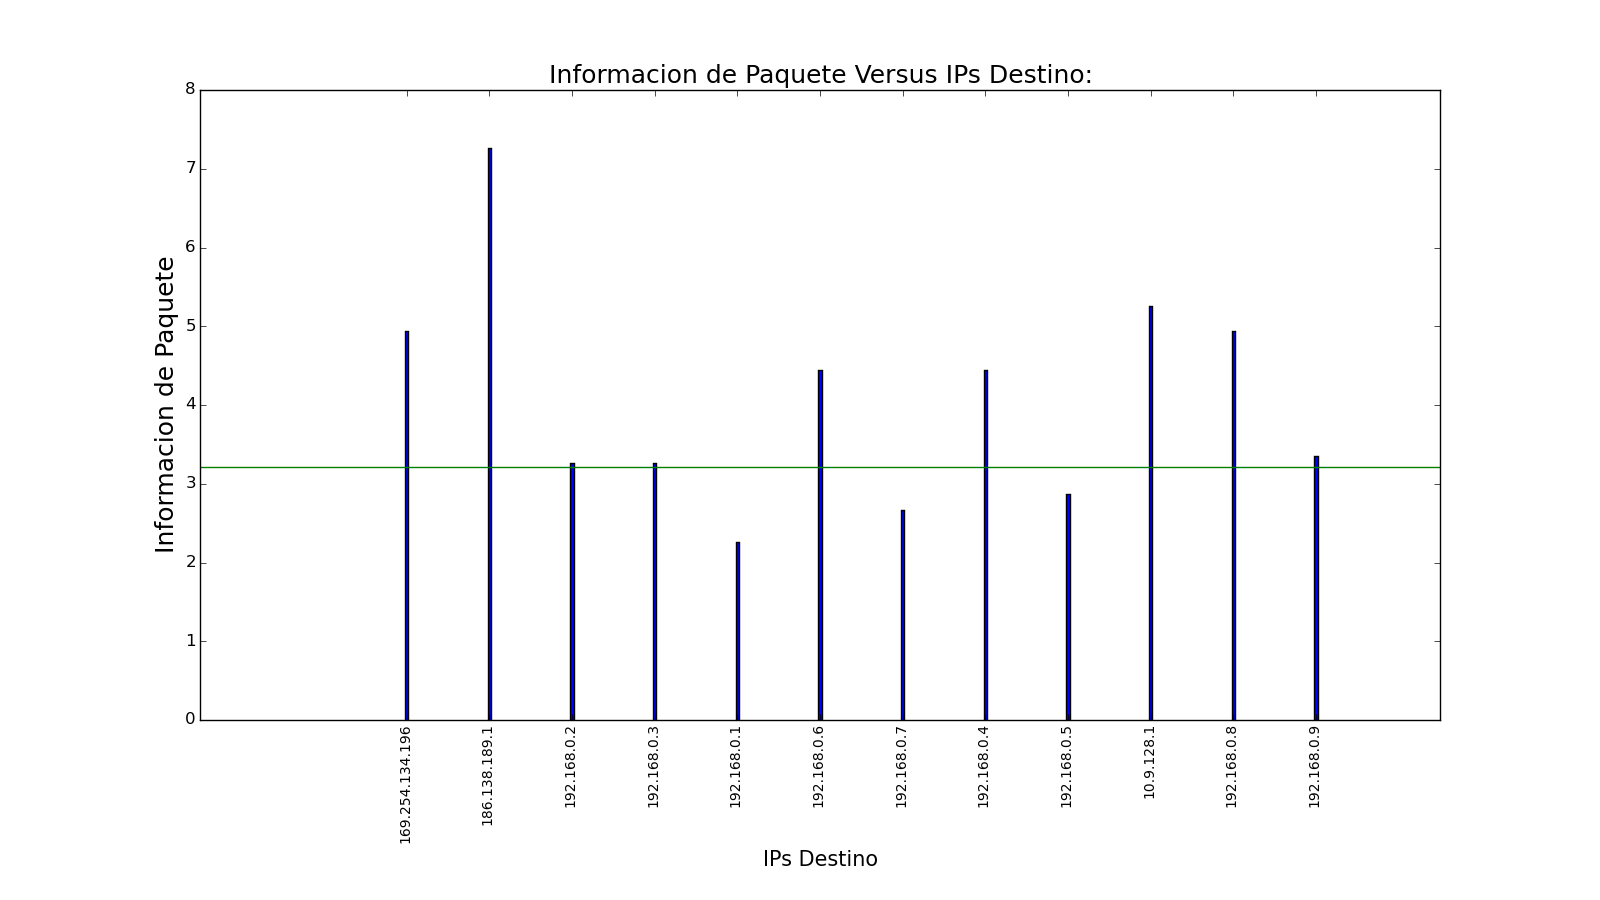
\includegraphics[width=1\textwidth]{../resultados/Casa/histogram_dst_information.png}
       \caption{Información de IPs destino de los paquetes ARP}
       \label{red-hogarena-arp-destination-info}
\end{figure}



\begin{figure}[H]
       \centering
       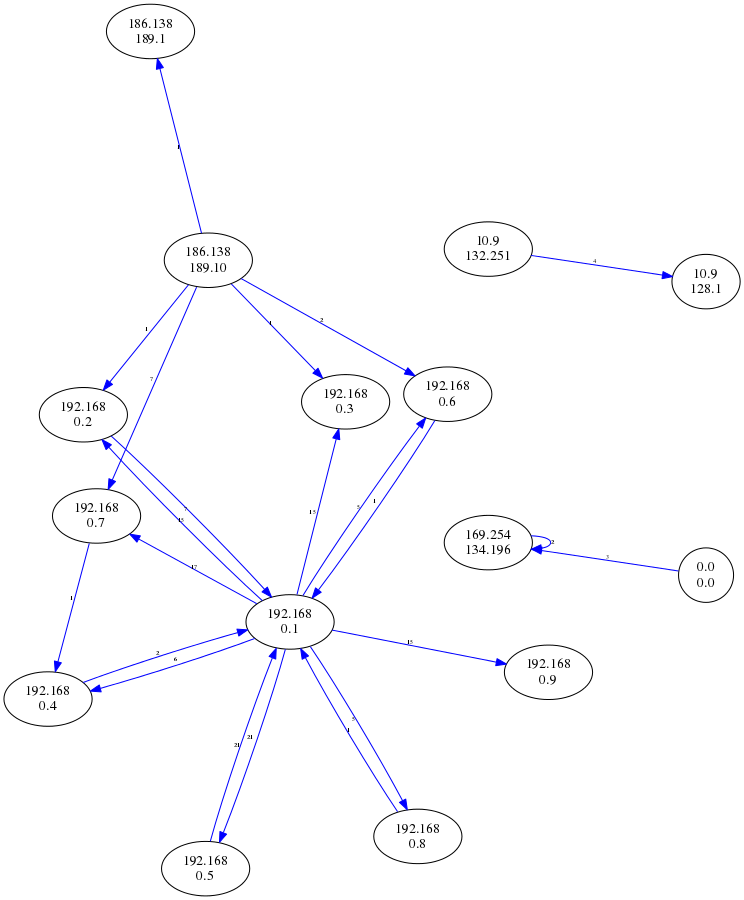
\includegraphics[width=1\textwidth]{../resultados/Casa/network.png}
       \caption{Tráfico de paquetes ARP}
       \label{red-hogarena-arp-traffic}
\end{figure}

Realizamos un gráfico del tráfico ARP de la red para ilustrar mejor los nodos distinguidos.
